\documentclass{beamer}
\usetheme{Malmoe}
\usepackage{minted}
\usepackage{hyperref}


\title[Kivy]{Kivy: a sweet new app development framework}
\author[Andy Wilson]{Andy Wilson}
\date[January 2012]{January 11, 2012}

\begin{document}
%--- the titlepage frame -------------------------%
\begin{frame}[plain]
  \titlepage
\end{frame}


\begin{frame}{hey who let you in here}
I'm Andy.

My level of experience:

I tried to do something with pygame once but got bored.

\end{frame}


\begin{frame}{the skinny}

\begin{itemize}
  \item Fast: OpenGL hardware accelerated goodness baked in
  \pause
  \item Easy: beautiful API
  \pause
  \item Multitouchtouchtouch
  \pause
  \item Crossplatform: Linux, Windows, OSX, Android
  \pause
  ...iOS (coming soon?)
  \pause
  \item License: LGPL3
\end{itemize}

\end{frame}


\begin{frame}{howsisworkthen?}
\begin{center}
  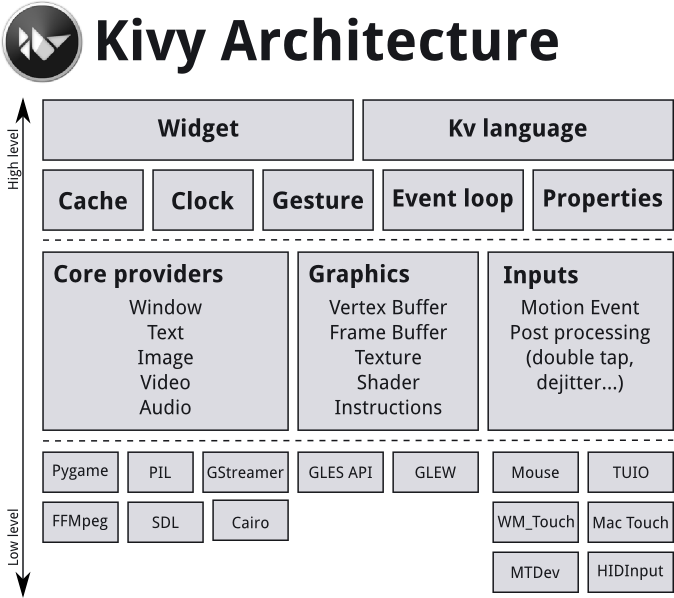
\includegraphics[height=.75\textheight]{architecture.png}
\end{center}

source: http://kivy.org/docs/guide/architecture.html

\end{frame}


\begin{frame}{widgets}

\begin{itemize}
  \item 
  \item use Kivy + pure python (no custom C or C extensions)
  \item put it on github
  \item ends Jan 31st (registration deadline: Jan 25th)
  \item prizes: android tablets, github subscriptions, t-shirts
\end{itemize}

\end{frame}



\begin{frame}[fragile]{hello world}
  \begin{minted}[linenos]{python}
    from kivy.app import App
    from kivy.uix.widget import Widget

    class HelloWidget(Widget):

        pass

    class WorldApp(App):
        def build(self):
            return HelloWidget()

    if __name__ == '__main__':
        WorldApp().run()

    TestApp().run()
  \end{minted}
\end{frame}



\begin{frame}{[CITATION NEEDED]}

Kivy project:  \url{http://kivy.org}

Source: \url{http://github.com/kivy/kivy}

Code/presentation: \url{http://github.com/wilsaj/flingy}

\end{frame}


\begin{frame}{two men enter one man leaves}

contest: \url{http://kivy.org/\#contest}

\begin{itemize}
  \item make a game
  \item use Kivy + pure python (no custom C or C extensions)
  \item put it on github
  \item ends Jan 31st (registration deadline: Jan 25th)
  \item prizes: android tablets, github subscriptions, t-shirts
\end{itemize}

\end{frame}


\end{document}